\documentclass{article}
\usepackage{graphicx}
\usepackage{amsmath}
\usepackage{amsfonts}
\usepackage{bookmark}
\usepackage{booktabs}
\usepackage{exercises}
\graphicspath{ {./images/5.6} }
\usepackage{indentfirst}
\usepackage{amsthm}
\usepackage{yhmath}
\usepackage{geometry}
\usepackage{placeins}
\usepackage{csquotes}
\usepackage{pgfplots}
\newcommand*{\oldneg}{\mathord{\sim}}
\newcommand\showdiv[1]{\overline{\smash{)}#1}}
\newcommand\Mydiv[1]{%
\smash{\raise.3ex\hbox{$\big)$}}\mkern-8mu
        \overline{\enspace\strut#1}}
\setlength{\tabcolsep}{5pt}
\theoremstyle{definition}
\newtheorem{definition}{Definition}

\setlength{\parindent}{.5in}
\setlength{\parskip}{12pt}
\renewcommand{\arraystretch}{2}
\geometry{margin=1in}
\newcommand{\?}{\stackrel{?}{=}}
\pgfplotsset{width=7cm,compat=1.18}\usepgfplotslibrary{statistics}

\title{5.6 Answers}
\begin{document}
\maketitle

\section*{1}
When you write $\frac{x}{3}=\frac{x+2}{5}$ as $5x=3(x+2)$, you are cross-multiplying.

\section*{2}
One can check for extraneous solutions by plugging them back into the original equation. In this case:
\[ \frac{5}{4-4}\?\frac{4}{4-4} \] \[ \frac{5}{0}\ne\frac{4}{0} \] as one cannot divide by zero, and:
\[ \frac{5}{5-4}\?\frac{5}{5-4} \] \[ 5=5 \] meaning $4$ is the extraneous solution.

\section*{3}
If one has a rational equation $p(x)=q(x)$, and thinks that $x_1$, say, is a solution of the equation, they could graph both $p(x)$ and $q(x)$. Then, if 
the two graphs intersect when $x=x_1$, the solution is not extraneous; if they don't intersect, it is extraneous.

\section*{10}
\[ \frac{x}{x^2-2}=\frac{-1}{x} \] \[ x^2=-x^2+2 \] \[ 2x^2=2 \] \[ x=\pm 1 \]
Check for extraneous solutions: \[ \frac{1}{1^2-2}\?\frac{-1}{1} \] \[ -1=-1 \] and \[ \frac{-1}{(-1)^2-2}\?\frac{-1}{-1} \] \[ 1=1 \] meaning both of $\pm 1$ are solutions.

\section*{11}
\[ \frac{4(x-4)}{x^2+2x-8}=\frac{4}{x+4} \] \[ 4(x-4)(x+4)=4(x^2+2x-8) \] \[ 4x^2-64=4x^2+8x-32 \] \[ 8x=-32 \] \[ x=-4 \]
Check for extraneous solutions: \[ \frac{4(-4-4)}{(-4)^2+2(4)-8}\?\frac{4}{-4+4} \] which is impossible as we cannot divide by zero.

\section*{13}
\[ \frac{3}{x+2}=\frac{6}{x-1} \] \[ 3x-3=6x+12 \] \[ x=-5 \]
A

\section*{16}
\[ \frac{5}{x}-2=\frac{2}{x+3} \] \[ x(x+3)(\frac{5}{x}-2)=\frac{2}{x+3}x(x+3) \] \[ 5x+15-2x^2-6x=2x \] \[ -2x^2-3x+15=0 \]
\[ -2x^2-3x=-15 \] \[ -2(x^2+\frac{3}{2}x)=-15 \] \[ -2(x^2+\frac{3}{2}x+\frac{9}{16})=-15-\frac{9}{8} \]
\[ -2(x+\frac{3}{4})^2=-\frac{129}{8} \]
\[ (x+\frac{3}{4})^2=\frac{129}{16} \]
\[ x+\frac{3}{4}=\pm\sqrt\frac{129}{16} \]
\[ x=-\frac{3}{4}\pm\frac{\sqrt{129}}{4}=\frac{-3\pm\sqrt{129}}{4} \]
Check for extraneous solutions:
\[ \frac{5}{\dfrac{-3+\sqrt{129}}{4}}-2\?\frac{2}{(\dfrac{-3+\sqrt{129}}{4})+3} \]
\[ \frac{20}{-3+\sqrt{129}}-2\?\frac{2}{\dfrac{9+\sqrt{129}}{4}} \]
\[ \frac{20(-3-\sqrt{129})}{(-3+\sqrt{129})(-3-\sqrt{129})}-2\?\frac{8}{9+\sqrt{129}} \]
\[ \frac{-60-20\sqrt{129}}{9-129}-2\?\frac{8(9-\sqrt{129})}{(9+\sqrt{129})(9-\sqrt{129})} \]
\[ \frac{-60-20\sqrt{129}}{-120}-2\?\frac{72-8\sqrt{129}}{81-129} \]
\[ \frac{3+\sqrt{129}}{6}-2\?\frac{-9+\sqrt{129}}{6} \]
\[ \frac{-9+\sqrt{129}}{6}=\frac{-9+\sqrt{129}}{6} \]
and
\[ \frac{5}{\dfrac{-3-\sqrt{129}}{4}}-2\?\frac{2}{(\dfrac{-3-\sqrt{129}}{4})+3} \]
\[ \frac{20}{-3-\sqrt{129}}-2\?\frac{2}{\dfrac{9-\sqrt{129}}{4}} \]
\[ \frac{20(-3+\sqrt{129})}{(-3+\sqrt{129})(-3-\sqrt{129})}-2\?\frac{8(9+\sqrt{129})}{(9-\sqrt{129})(9+\sqrt{129})} \]
\[ \frac{-60+20\sqrt{129}}{-120}-2\?\frac{72+8\sqrt{129}}{-48} \]
\[ \frac{3-\sqrt{129}}{6}-2\?\frac{-9-\sqrt{129}}{6} \]
\[ \frac{-9-\sqrt{129}}{6}=\frac{-9-\sqrt{129}}{6} \] 
meaning neither of the solutions are extraneous.

\section*{17}
\[ \frac{1}{2x}+\frac{3}{x+7}=\frac{-1}{x} \] \[ 2x(x+7)(\frac{1}{2x}+\frac{3}{x+7})=\frac{-1}{x}2x(x+7) \]
\[ x+7+6x=-2x-14 \] \[ 9x=-21 \] \[ x=-\frac{21}{9}=-\frac{7}{3} \]
Check for extraneous solutions:
\[ \frac{1}{2\frac{-7}{3}}+\frac{3}{-\frac{7}{3}+7}\?\frac{-1}{-\frac{7}{3}} \]
\[ \frac{3}{-14}+\frac{9}{14}\?\frac{-1}{-\frac{7}{3}} \]
\[ \frac{3}{7}=\frac{3}{7} \]
Meaning there is no extraneous solution.

\section*{23}
\[ \frac{10}{x}+3=\frac{x+9}{x-4} \] \[ x(x-4)(\frac{10}{x}+3)=\frac{x+9}{x-4}x(x-4) \]
\[ 10x-40+3x^2-12x=x^2+9x \] \[ 2x^2-11x-40=0 \] \[ (2x+5)(x-8)=0 \] \[ x=-\frac{5}{2}\vee 8 \]
Check for extraneous solutions:
\[ \frac{10}{-\frac{5}{2}}+3\?\frac{-\frac{5}{2}+9}{-\frac{5}{2}-4} \] \[ -4+3\?-\frac{\frac{13}{2}}{\frac{13}{2}} \] \[ -1=-1 \]
and \[ \frac{10}{8}+3\?\frac{8+9}{8-4} \] \[ \frac{5}{4}+3\?\frac{17}{4} \] \[ \frac{17}{4}=\frac{17}{4} \]
meaning there are no extraneous solutions.

\section*{28}
\[ \frac{2}{x-3}=\frac{1}{x^2-2x-3} \] \[ 2(x^2-2x-3)=x-3 \] \[ 2x^2-4x-6=x-3 \] \[ 2x^2-5x-3=0 \] \[ (2x+1)(x-3)=0 \] \[ x=-\frac{1}{2}\vee 3 \]
Check for extraneous solutions:
\[ \frac{2}{-\frac{1}{2}-3}\?\frac{1}{(-\frac{1}{2})^2-2(-\frac{1}{2})-3} \]
\[ -\frac{4}{7}\?\frac{1}{-\frac{7}{4}} \] \[ -\frac{4}{7}=-\frac{4}{7} \]
and \[ \frac{2}{3-3}\?\frac{1}{3^2-2(2)-3} \] which is impossible, as we cannot divide by zero. Thus $-\frac{1}{2}$ is the only solution.
C

\section*{30}
We first solve the equation:
\[ \frac{1}{x-a}=\frac{x}{x-a} \] \[ x=1 \] 
Thus the statement is sometimes true. For example, it could be that $a=1$, meaning, although $x=1=a$ is a solution, it is 
extraneous as we cannot divide by $1-1=0$.

\section*{31}
We solve the equation:
\[ \frac{3}{x-a}=\frac{x}{x-a} \] \[ x=3 \] Thus the statement that the equation has exactly one solution is sometimes true. It could be false if the equation has no solutions, for example, 
if $a=3$.


\section*{32}
We solve the equation:
\[ \frac{1}{x-a}=\frac{2}{x+a}+\frac{2a}{x^2-a^2} \]
\[ \frac{1}{x-a}=\frac{2}{x+a}+\frac{2a}{(x+a)(x-a)} \]
\[ (x+a)(x-a)\frac{1}{x-a}=(\frac{2}{x+a}+\frac{2a}{(x+a)(x-a)})(x+a)(x-a) \]
\[ x+a=2x-2a+2a \]
\[ x=a \] This shows that the statement that the equation has no solution is always true. For, $x$ cannot equal $a$, or else we would be dividing by $x-x=0$, which is impossible.

\section*{37}
We know that $\frac{w}{l}=\frac{l}{l+w}$. If $w=1$, then:
\[ \frac{1}{l}=\frac{l}{l+1} \] \[ l+1=l^2 \] \[ l^2-l=1 \] \[ l^2-l+(\frac{1}{2})^2=1+(\frac{1}{2})^2 \]
\[ (l-\frac{1}{2})^2=\frac{5}{4} \]
\[ l-\frac{1}{2}=\pm\frac{\sqrt{5}}{2} \]
\[ l=\frac{1}{2}\pm\frac{\sqrt{5}}{2}=\frac{1\pm\sqrt{5}}{2}\approx -0.618\vee 1.618 \]
Because the ratio of the length to the width cannot be negative, $-0.618$ can be ruled out, meaning the golden ratio is $\frac{1+\sqrt{5}}{2}$, 
or about $1.618$.

\section*{38}
(This question was unclear. Does $h(x)$ represent the average number of minutes per month, or per year? I assumed it was per month.)\newline
(a): We are given $g(x)$, the average monthly bill for mobile phone users, and $h(x)$, the average number of minutes per month used by U.S. mobile phone users $x$ years after 1998. Thus the average
price per minute is
$\frac{g(x)}{h(x)}$, or:
\[ f(x)=\dfrac{-0.27x^3+1.40x^2+1.05x+39.4}{-8.25x^3+53.1x^2-7.82x+138} \]


(b): Plugging in 0 to the above equation (for 1998, that is, 0 years after 1998), yields $\approx \$0.29$ per minute.


(c): \newline 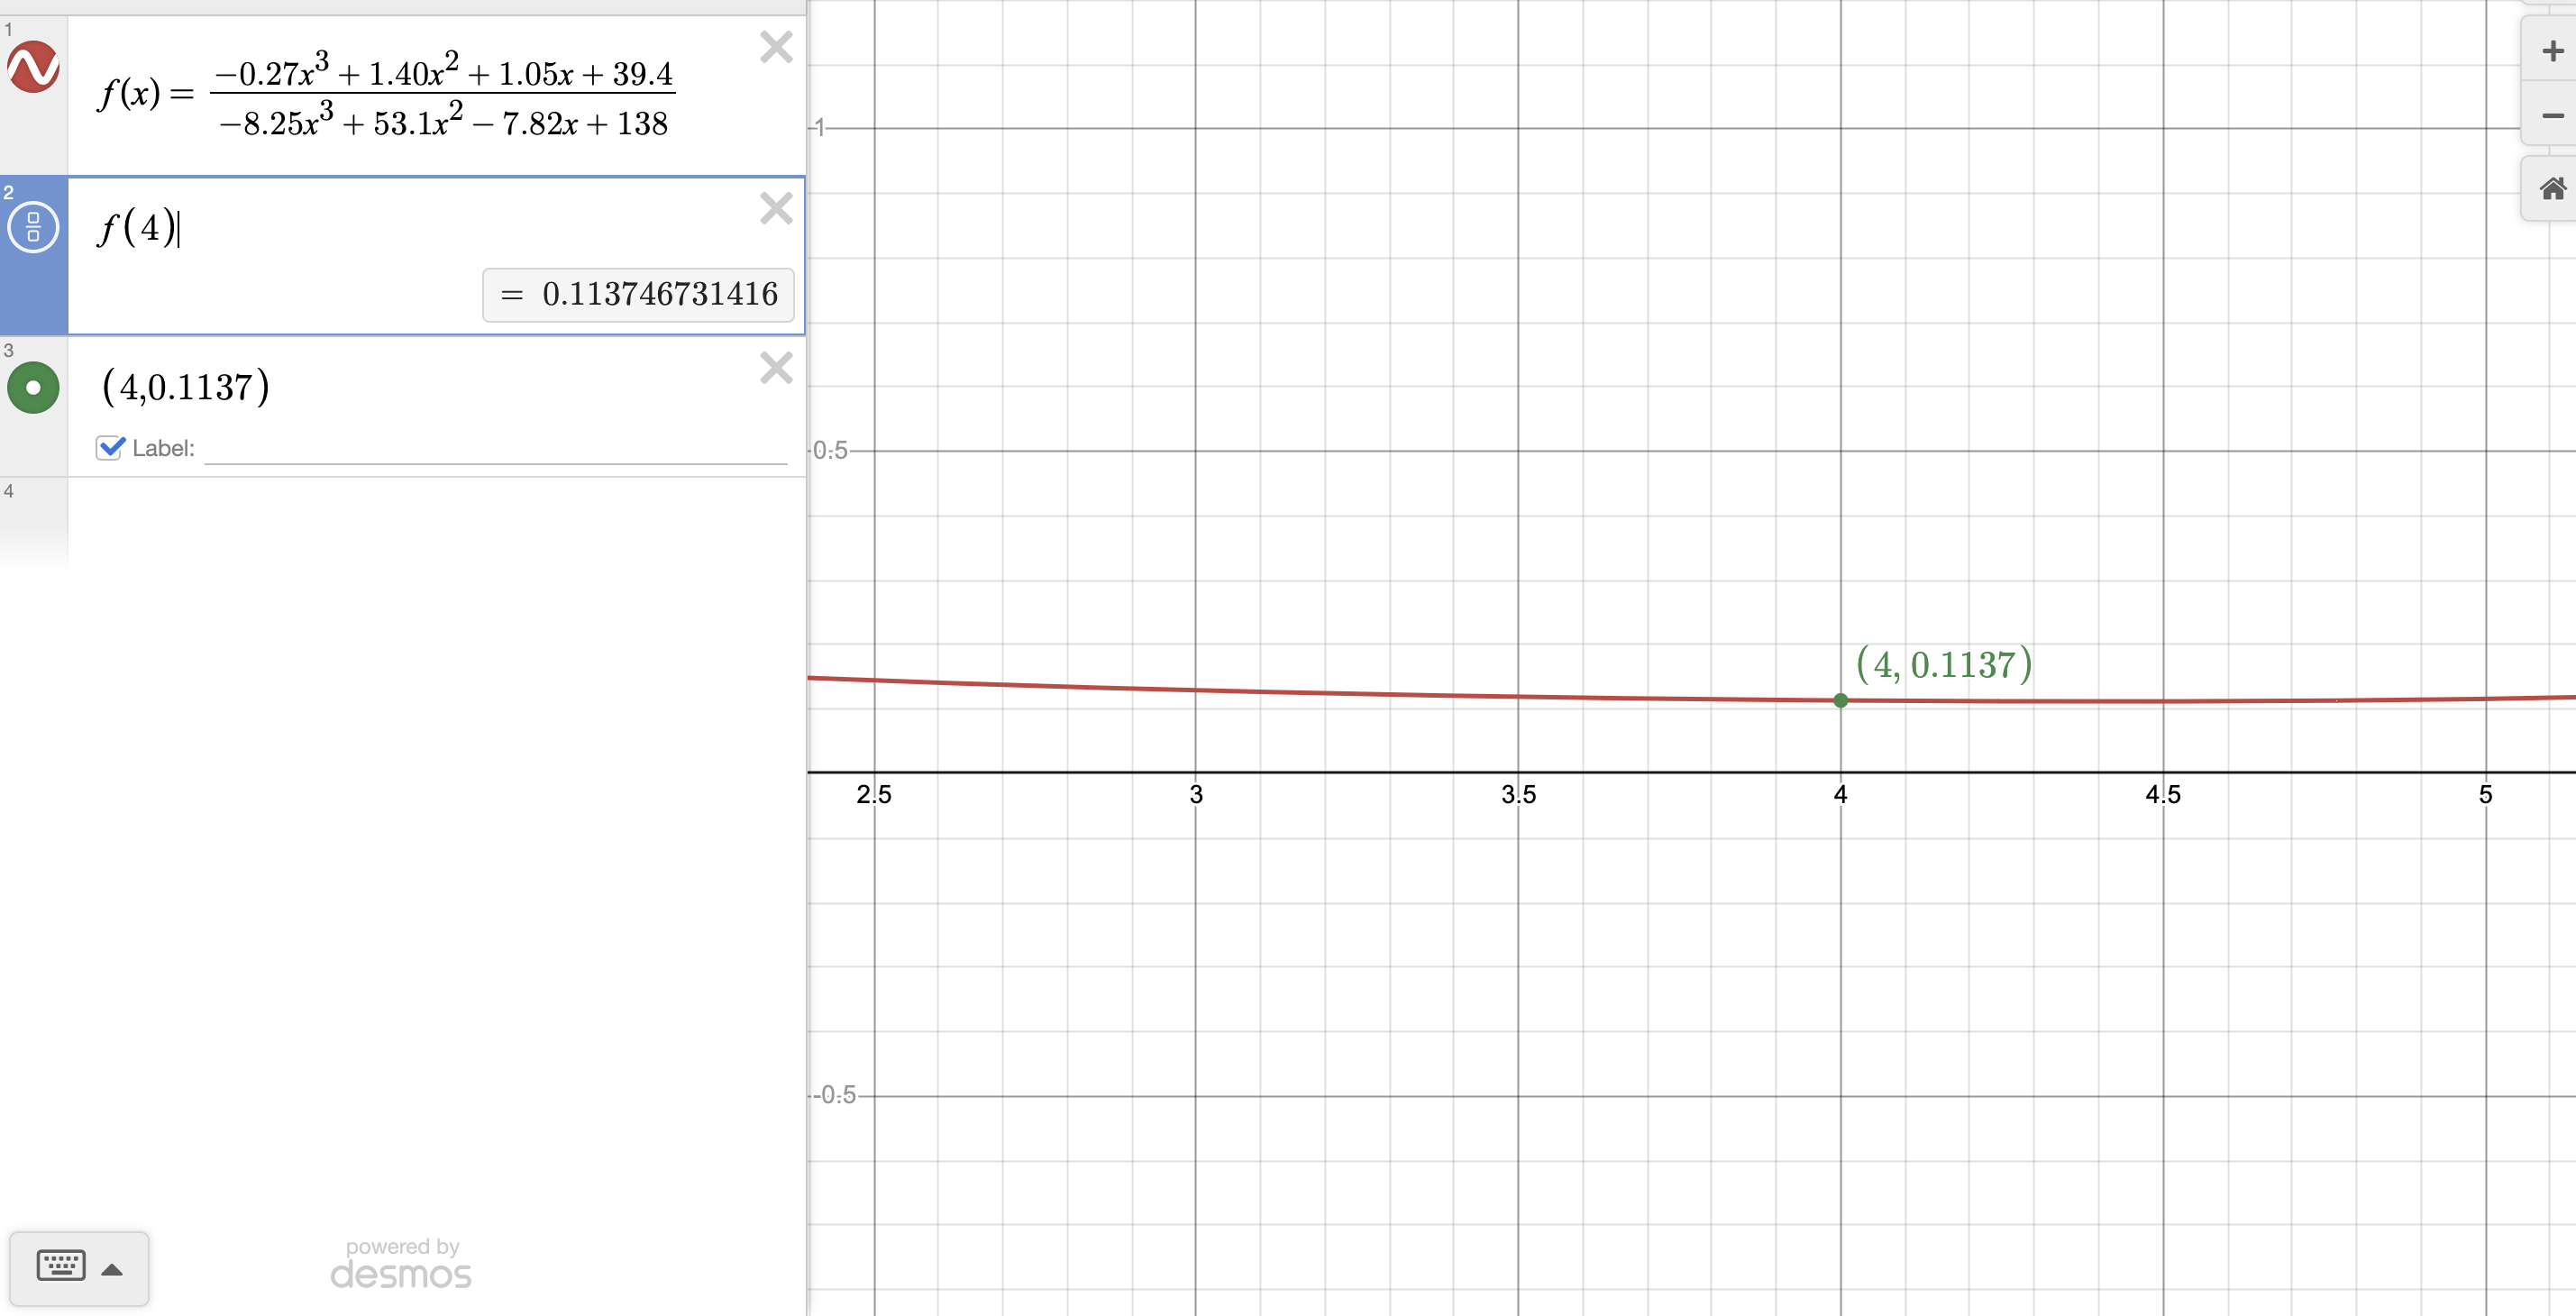
\includegraphics[width = 4in, height = 4in]{38}\newline 
From the graph, we can see that the average price per minute fell to about 11 cents 4 years after 1998, that is, in 2002. 

\end{document}
